\documentclass{article}
\usepackage{geometry}
\usepackage[utf8]{inputenc}
\usepackage{graphicx}
\graphicspath{ {images/} }
\geometry{a4paper, total={170mm,257mm}, left=25mm, right=25mm, top=25mm, bottom=25mm}
\setlength{\parindent}{2em}
\setlength{\parskip}{1em}
\renewcommand{\baselinestretch}{1.3}

\title{FOAR705 - S.Goldie Learning Journal}
\author{Sheriden Goldie}
\date{9th August 2019}

\begin{document}

\maketitle

\section*{Using LaTeX to create a document}

\textbf{Aims:}
\begin{itemize}
    \item familiarise myself with document creation system
    \item create entry for learning journal
    \end{itemize}

\textbf{Resources:}
\begin{itemize}
    \item Overleaf for LaTeX - Online editor
    \item Overleaf guide - 
    \end{itemize}
\begin{verbatim} https://www.overleaf.com/learn/latex/Learn_LaTeX_in_30_minutes \end{verbatim}

\textbf{Expectations:}
\begin{itemize}
    \item The guide claims to be able to teach me how to cover the basics of LaTeX in 30 minutes
    \item That I will be able to create a document, and replicate this process on my own without the guide
\end{itemize}


\section*{Experience/Errors}

When copying in code from the guide, I duplicated a line which had additional information. The error was highlighted when I tried to recompile the document and I noted that the changes I expected had not been made.
See figure \ref{fig:screenshot1}.

I removed the first line of code instead of the highlighted one – as I considered that while the highlighted was the second instance but had the more relevant information in it.

I continued following the instructions. See figure \ref{fig:screenshot2}.
I was confused as to why the title/author information wasn’t appearing on the document and spent too long re-reading that section. When I looked at the next section of the guide this was resolved using the "maketitle" code line.

See figure \ref{fig:screenshot3} for error when inserting an image.
This was due to the image being to wide for the page dimensions set in the preamble. 
I was able to fix this by changing the specified width of the image.
I tried a more basic way to include the image – and had a similar error see figure \ref{fig:screenshot4}.

This confused me, until I looked at the preview screen. As the program is interpreting the code directly – it is not adding the line break space between text and line. Once I added a line this problem was resolved. 

In following the guide, I tried adding a figure – but it didn’t appear when I recompiled. I realised I had entered the code below the tag - \begin{verbatim}\end{document}\end{verbatim} See figure \ref{fig:screenshot5}.

Inserting the figure wasn’t working. The text and the image were separating – the text was above the image when I wanted it below.
See figure \ref{fig:screenshot6}.
I wasn’t sure how to fix it – so I viewed an example template on overleaf – this was super helpful – and it showed me that the documents for the project on the left could be nested in folders – thus explaining the graphic path line of code for the image registry folder. So I applied this in my document as well. 
See figure \ref{fig:overleaf}.

However I was still having issues with the image and text appearing in an order contrary to my desire, and I had an error with the cross references I was trying to create. 
See figure \ref{fig:screenshot7}.

I read the log error and realised the issue with the cross references was I had change the label for the figure – and so the reference wasn’t linking to anything it could find. 
See figure \ref{fig:screenshot8}.

The issue with the image ordering etc – comes from the “float” directive. The letters following the tag: \begin{verbatim}
    \begin{figure}[*]
\end{verbatim}  indicate how the document will place the image * here can be various indicators.
Changing these on my figures doesn’t solve my problem
I added a page break tag:
\begin{verbatim}
    \pagebreak
\end{verbatim} 
I added this under my first image – as well as changing the float indicators to ‘h’ – this seemed to fix the problem – though I’m not sure its foolproof. 

The next step was to create lists in the document.
When I first did this the bold text tag didn’t work when a capital letter was included. 
 See figure \ref{fig:screenshot9}.
I also tried using the section and subsection tags. 

I tired different text formatting options:
See figure \ref{fig:screenshot10}.

I tried sections etc and the chapter tag didn’t work – this I found is because this is only available in “book” or “report” document classes. 
See figure \ref{fig:screenshot11}.


\section*{Reflections}

So this process did not take 30minutes – this took me closer to an hour – partly because I was documenting the process – but also because all did not go as quickly when I was actively trying to understand how this system worked.

Creating the actual learning journal document then took significantly longer as well - as I was implementing a wider scope of actions compared to the practice. 

When I begin to create the learning journal document using LaTeX – I continue to have issues with image placement in relation to text and the ordering of such objects. So I placed all the images in their own section and utilised the cross referencing. This is not my preference for this kind of document - but it is fit enough for purpose at this stage. 

I also experienced my first "fatal" errors that prevented the document compiling at all - these were scary at first. Then I found with the language I had been learning through the tutorial, and my own practice I was able to understand the error. I generally fixed this by first removing the code/element I had been trying to add/create, and closely examine what i was trying to do and how - rereading notes and guides on doing so. 

Ultimately I was able to learn to create a document using LaTeX. However, I wasn't able to immediately complete another document unassisted. New problems occurred, which required checking previous notes and further guides. Certainly I think this will be a factor of using this new system for quite some time, and filtering the relevant information can be difficult as well. 

I still have a problem with the formatting on my first page with the alignment of paragraphs under the word "Aims:". I think this is a problem I will need to take to my teachers for more insight - as I have not found a solution through my guides.


\pagebreak
\section*{Figures}

\begin{figure}[h]
    \centering
    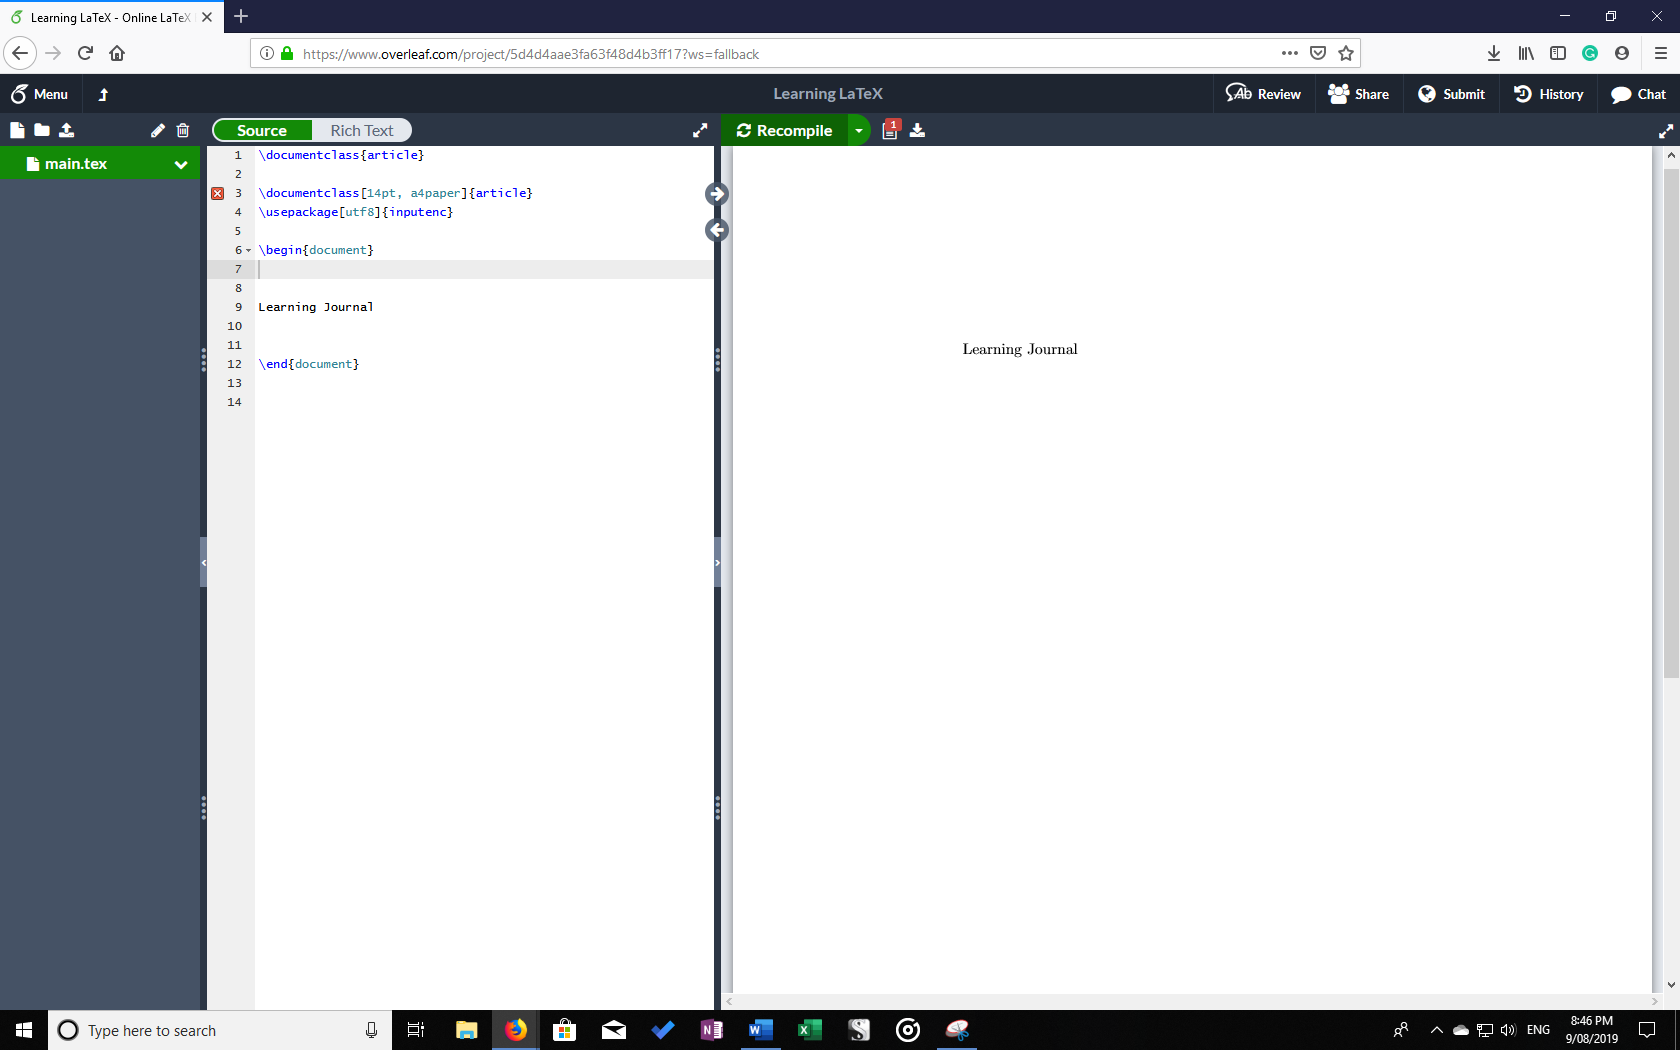
\includegraphics[width=12cm]{Images/Screenshot1.png}
    \caption{My first LaTeX Error}
    \label{fig:screenshot1}
\end{figure}

\begin{figure}[h]
    \centering
    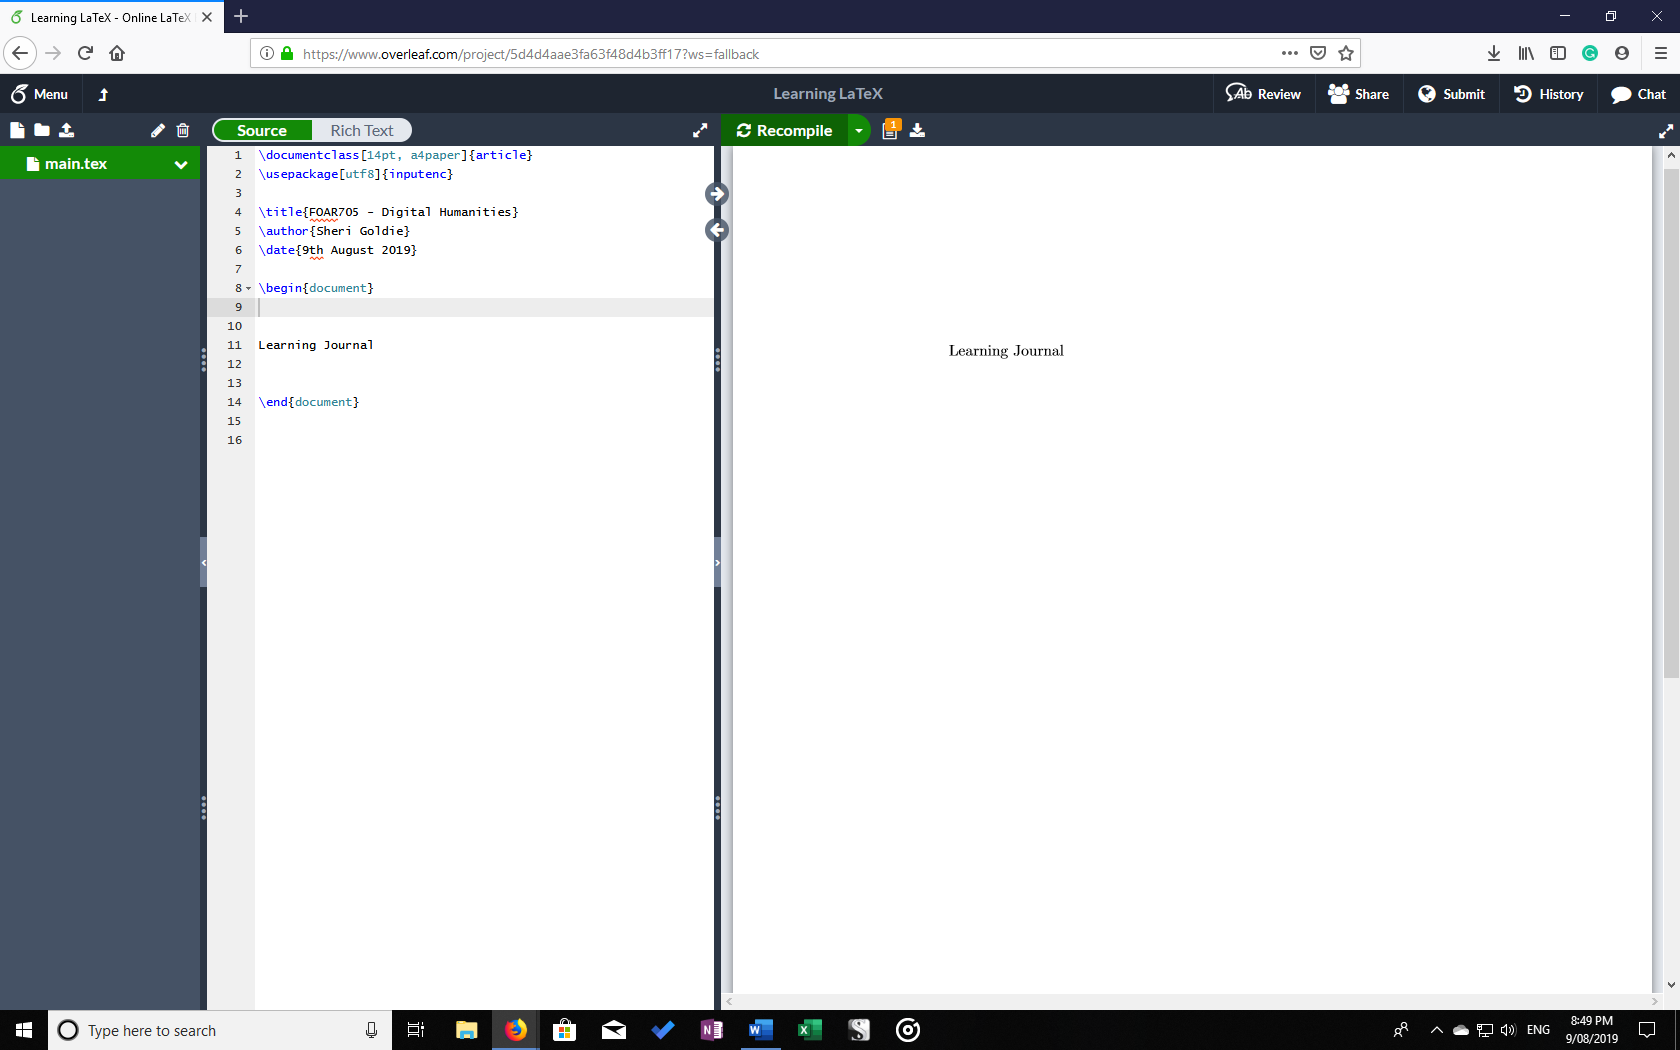
\includegraphics[width=12cm]{Images/Screenshot2.png} 
    \caption{Problem still present}
    \label{fig:screenshot2}
\end{figure}

\begin{figure}[h]
    \centering
    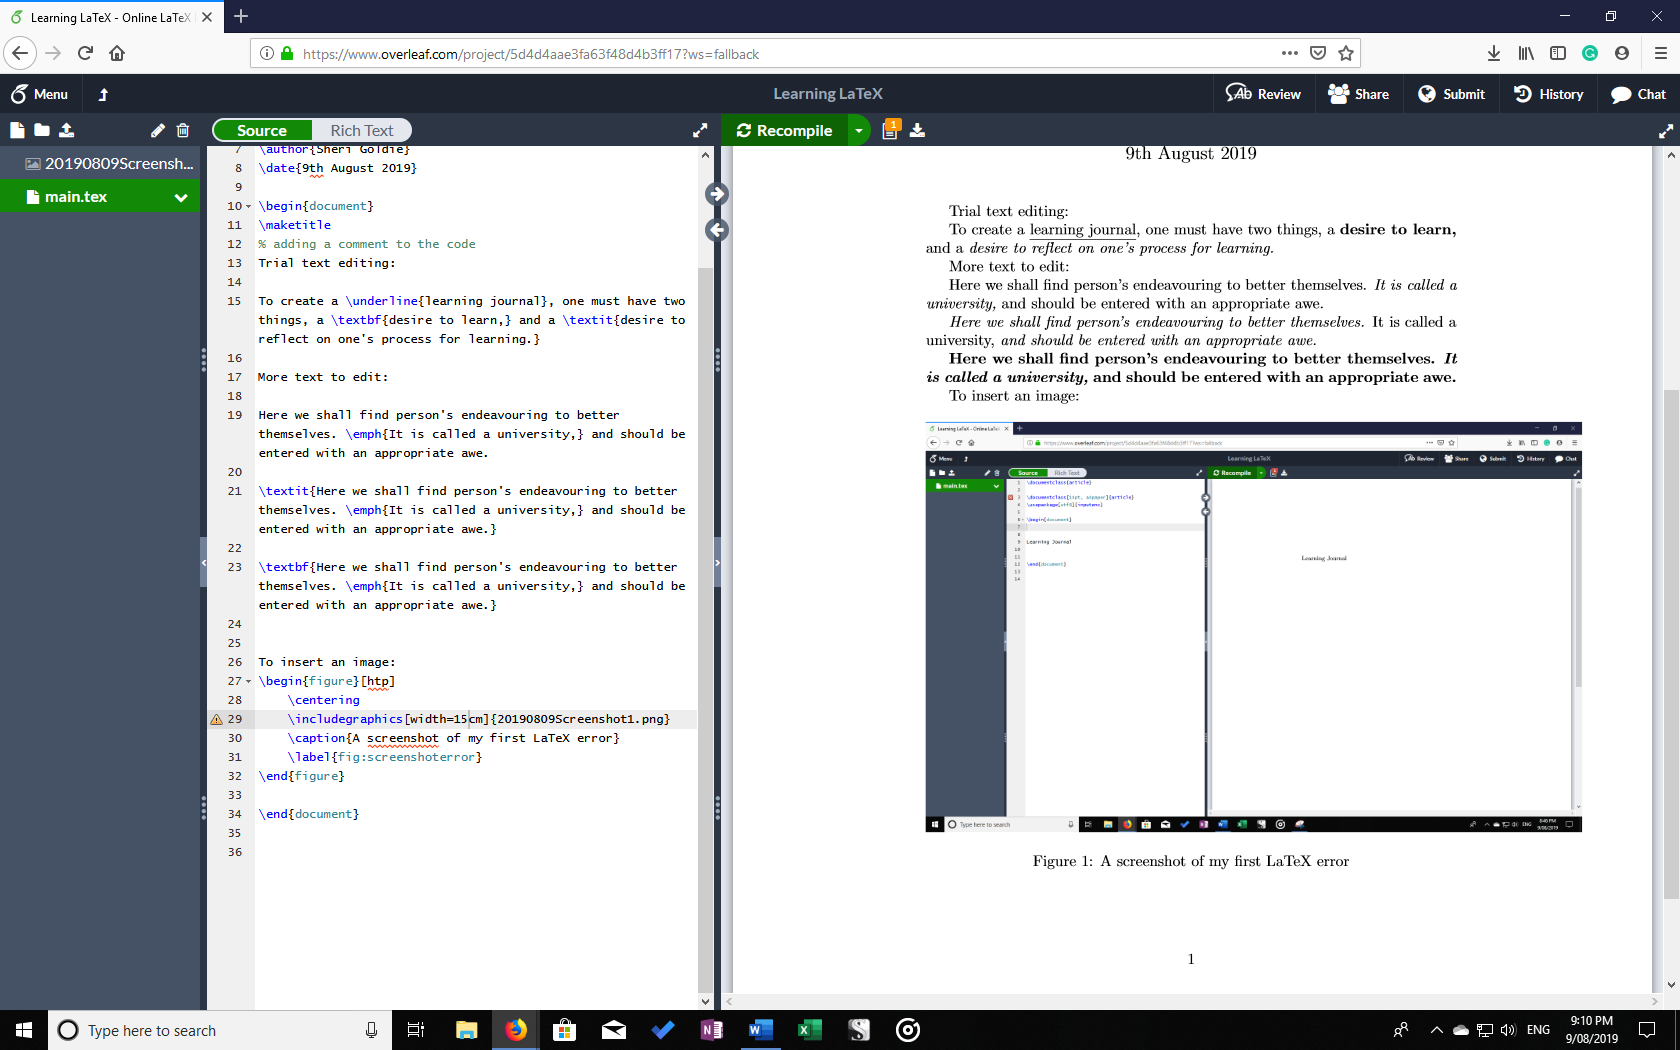
\includegraphics[width=12cm]{Images/Screenshot3.png}
    \caption{Image errors}
    \label{fig:screenshot3}
\end{figure}

\begin{figure}[h]
    \centering
    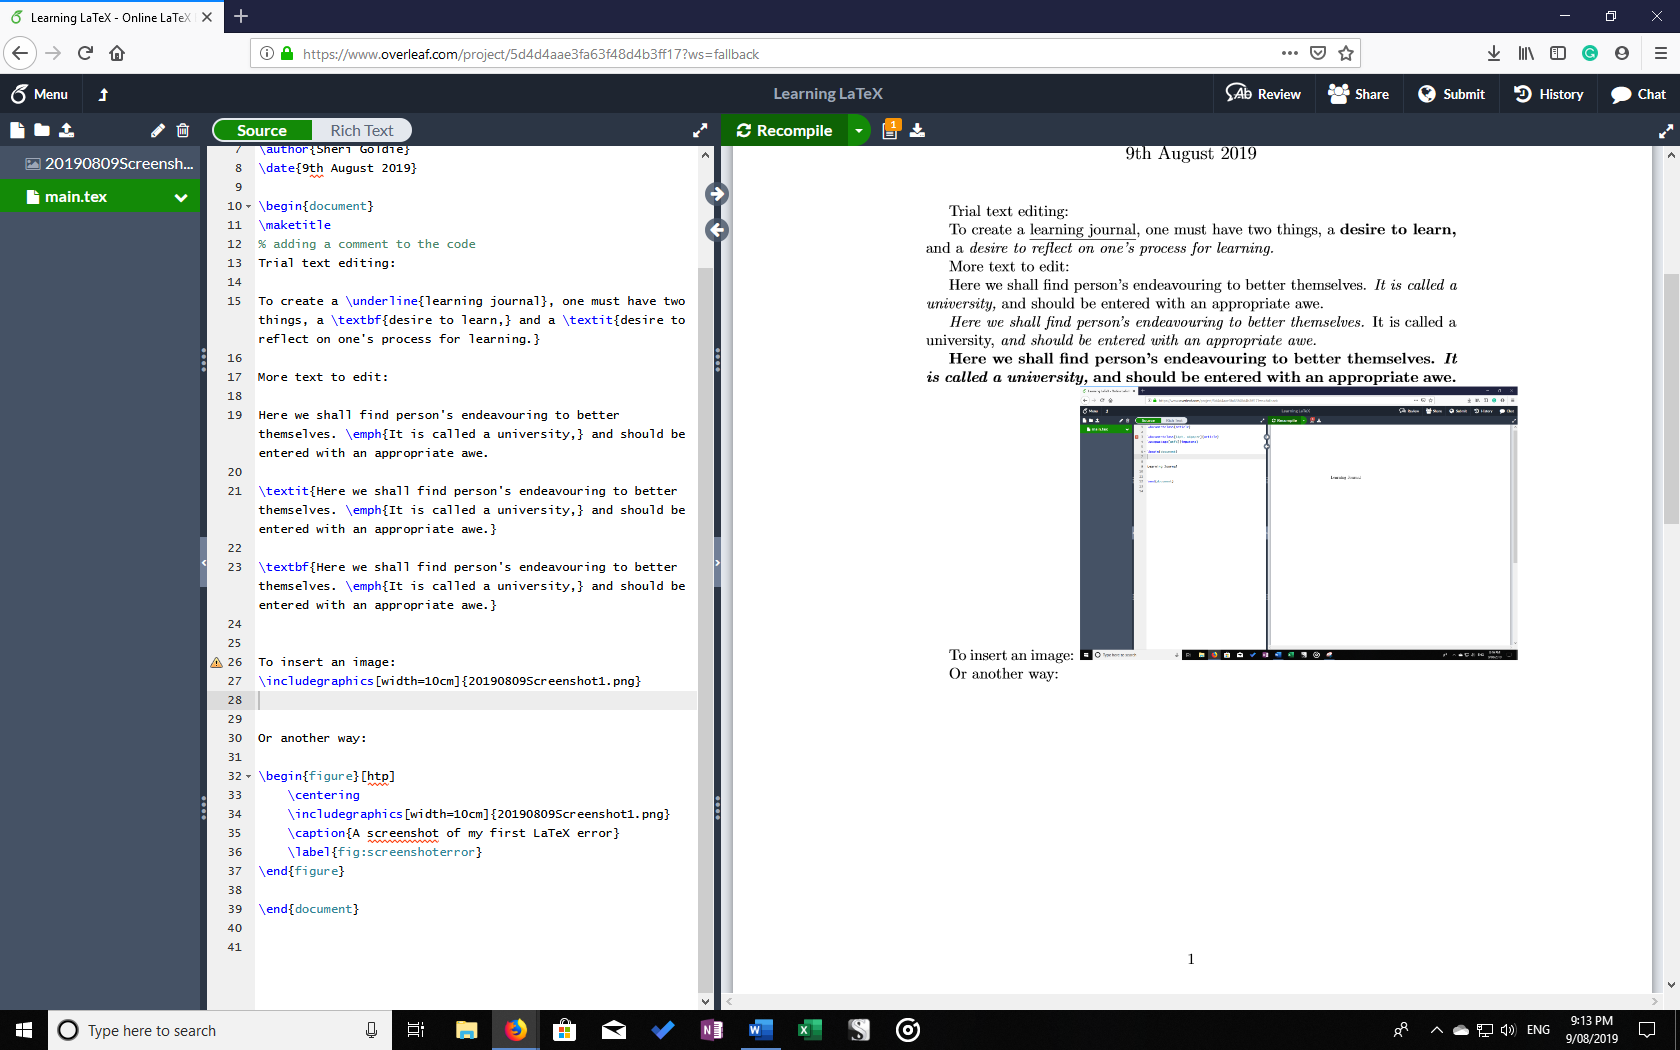
\includegraphics[width=12cm]{Images/Screenshot4.png}
    \caption{Image Errors 2}
    \label{fig:screenshot4}
\end{figure}

\begin{figure}[h]
    \centering
    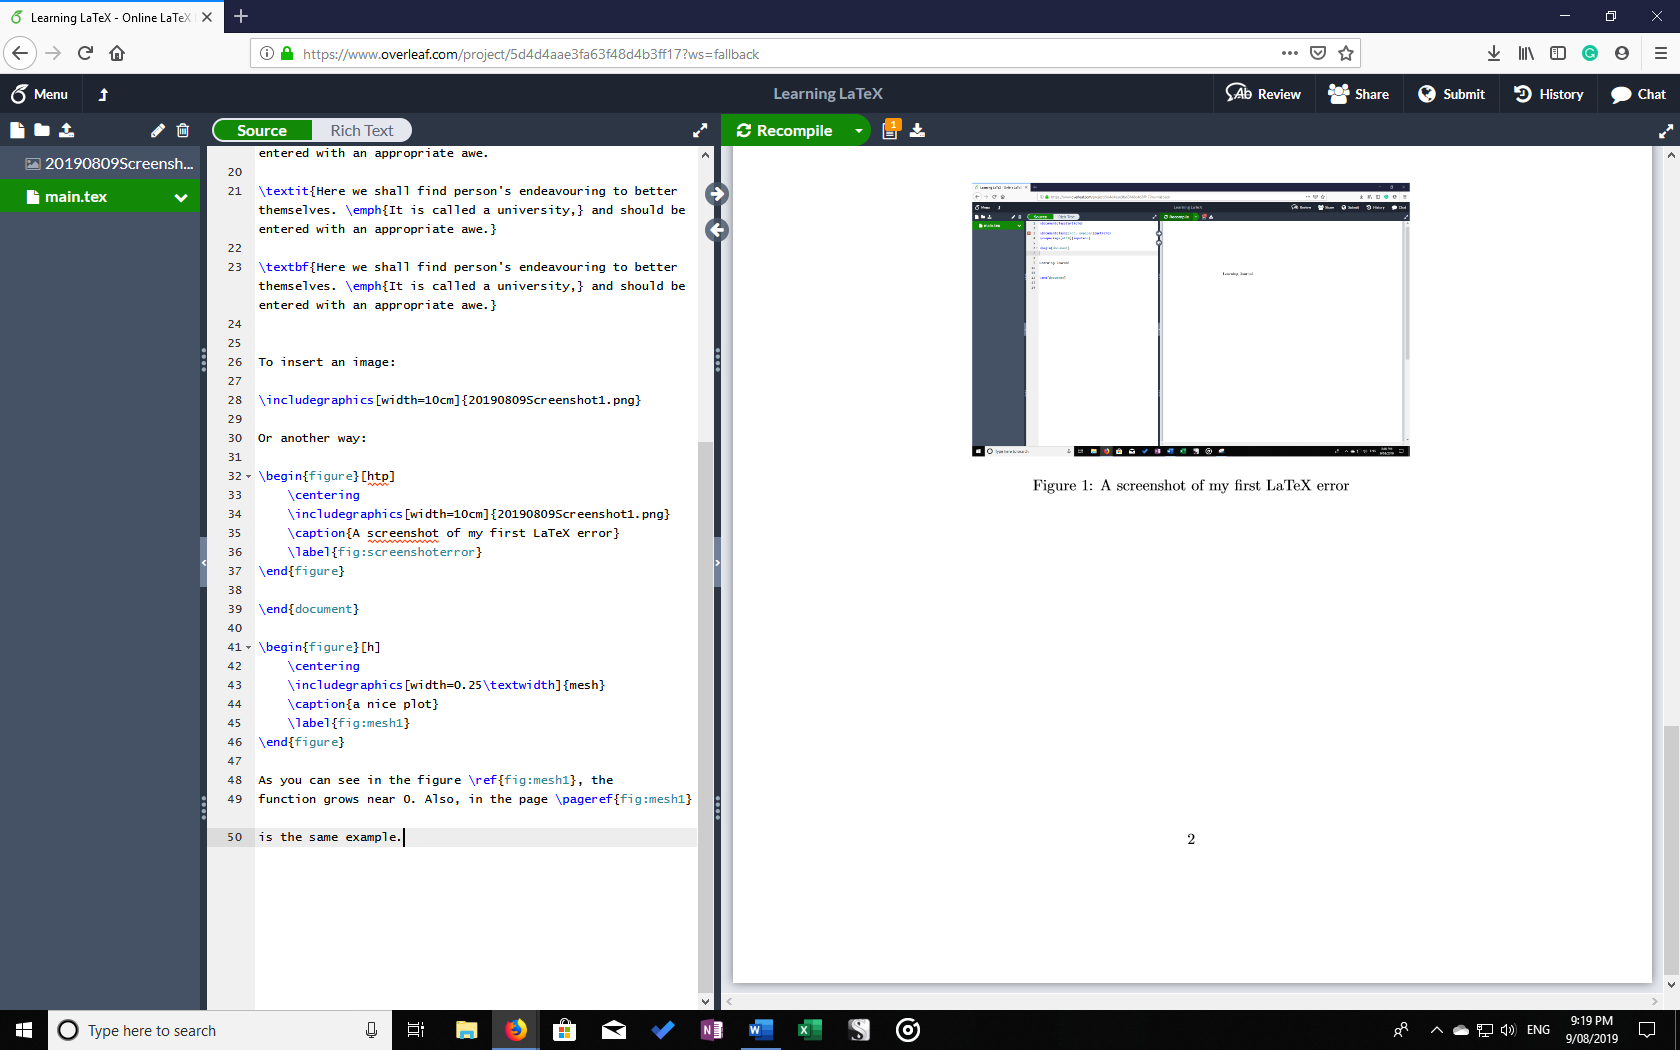
\includegraphics[width=12cm]{Images/Screenshot5.png}
    \caption{Element placed below end document tag}
    \label{fig:screenshot5}
\end{figure}

\begin{figure}[h]
    \centering
    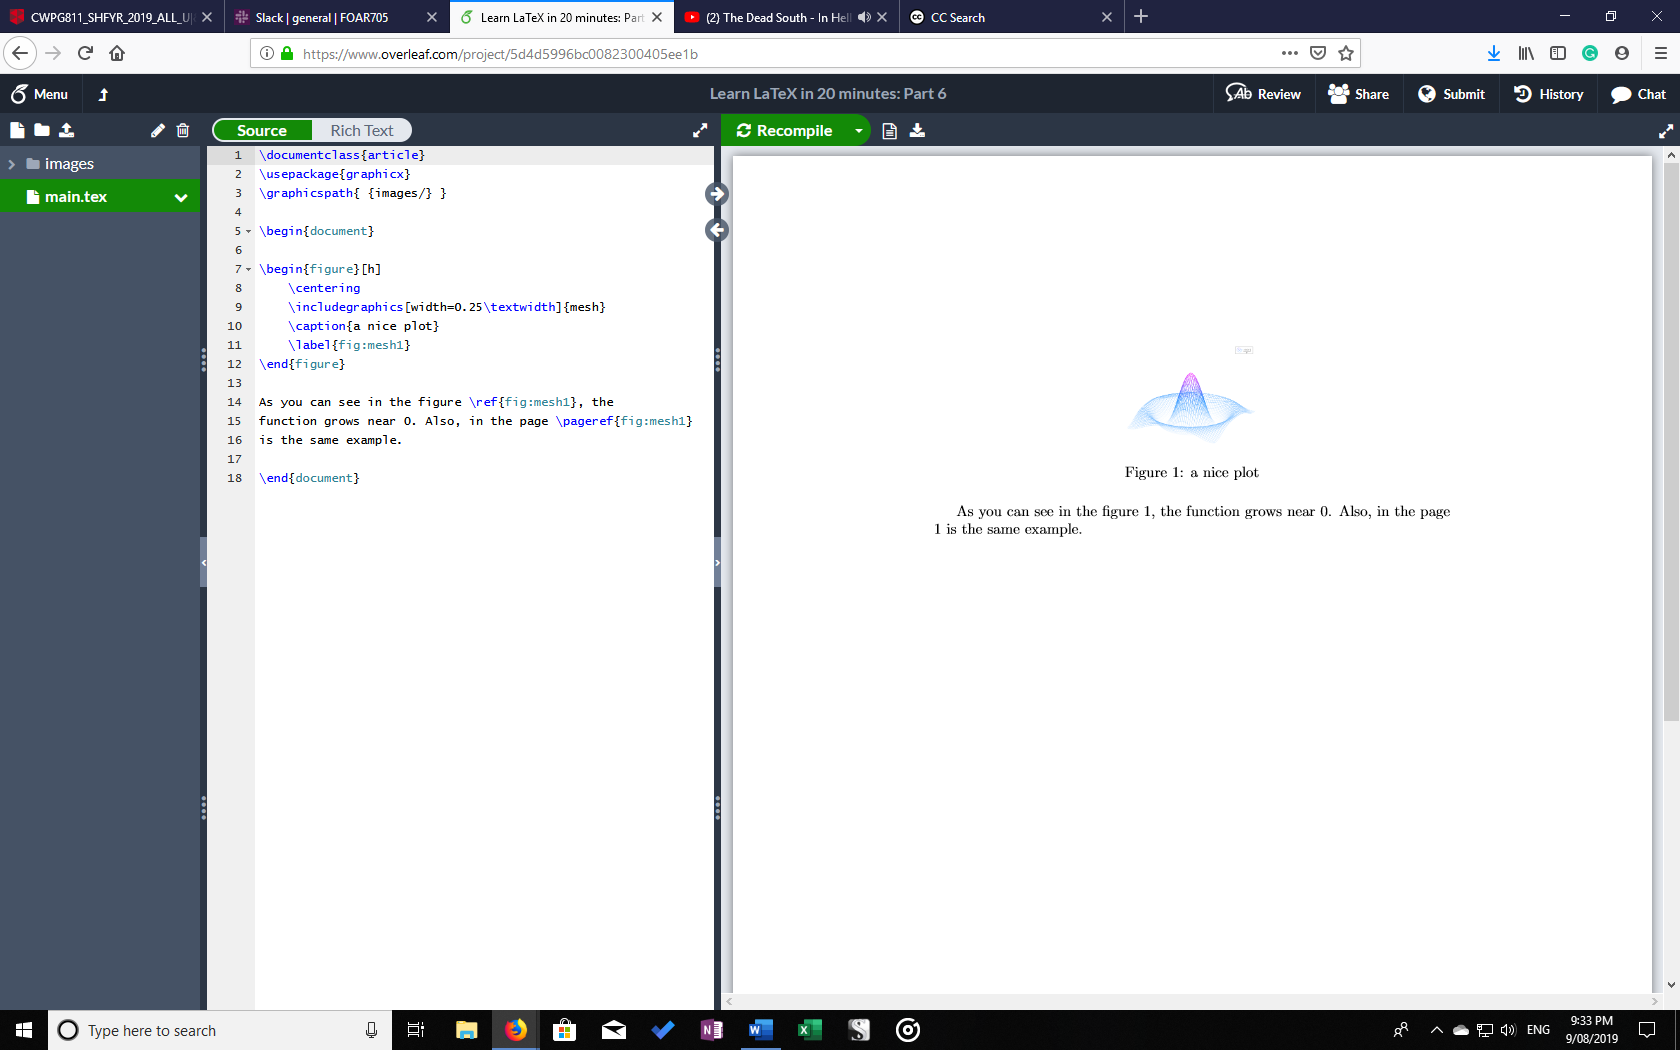
\includegraphics[width=12cm]{Images/OverleafExample.png}
    \caption{Example document from Overleaf tutorial}
    \label{fig:overleaf}
\end{figure}

\begin{figure}[h]
    \centering
    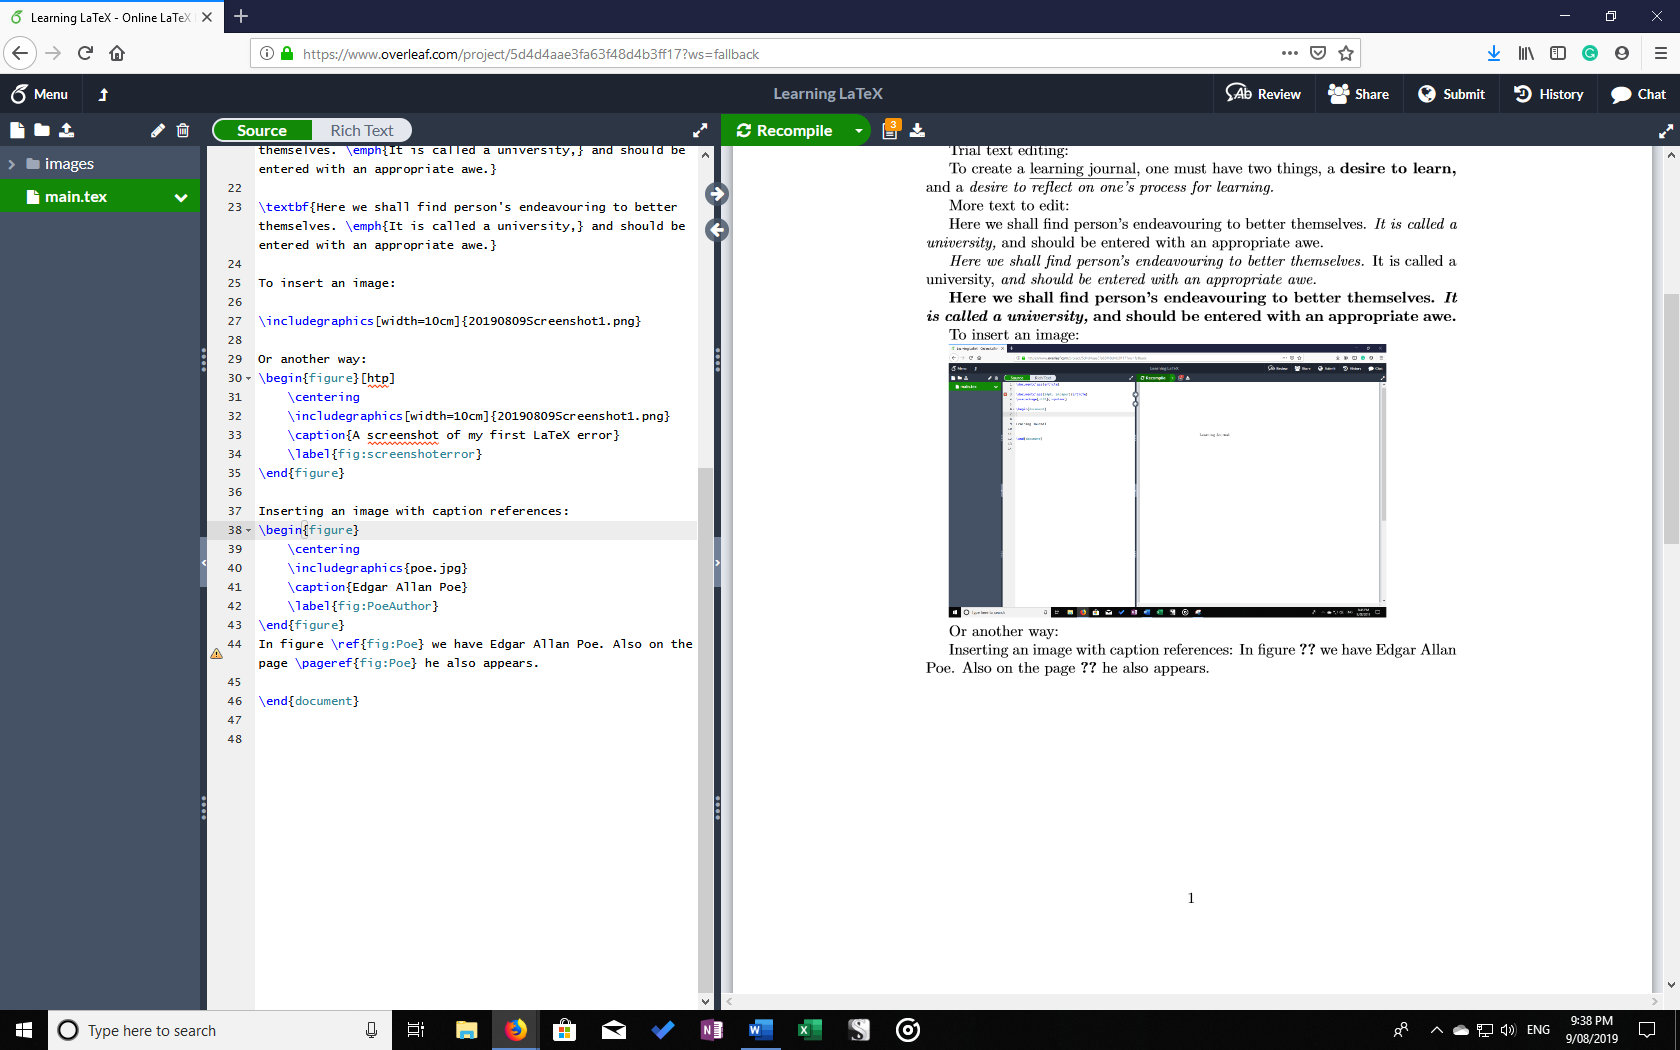
\includegraphics[width=12cm]{Images/Screenshot6.png}
    \caption{Labeling Figures properly}
    \label{fig:screenshot6}
    \end{figure}

\begin{figure}[h]
    \centering
    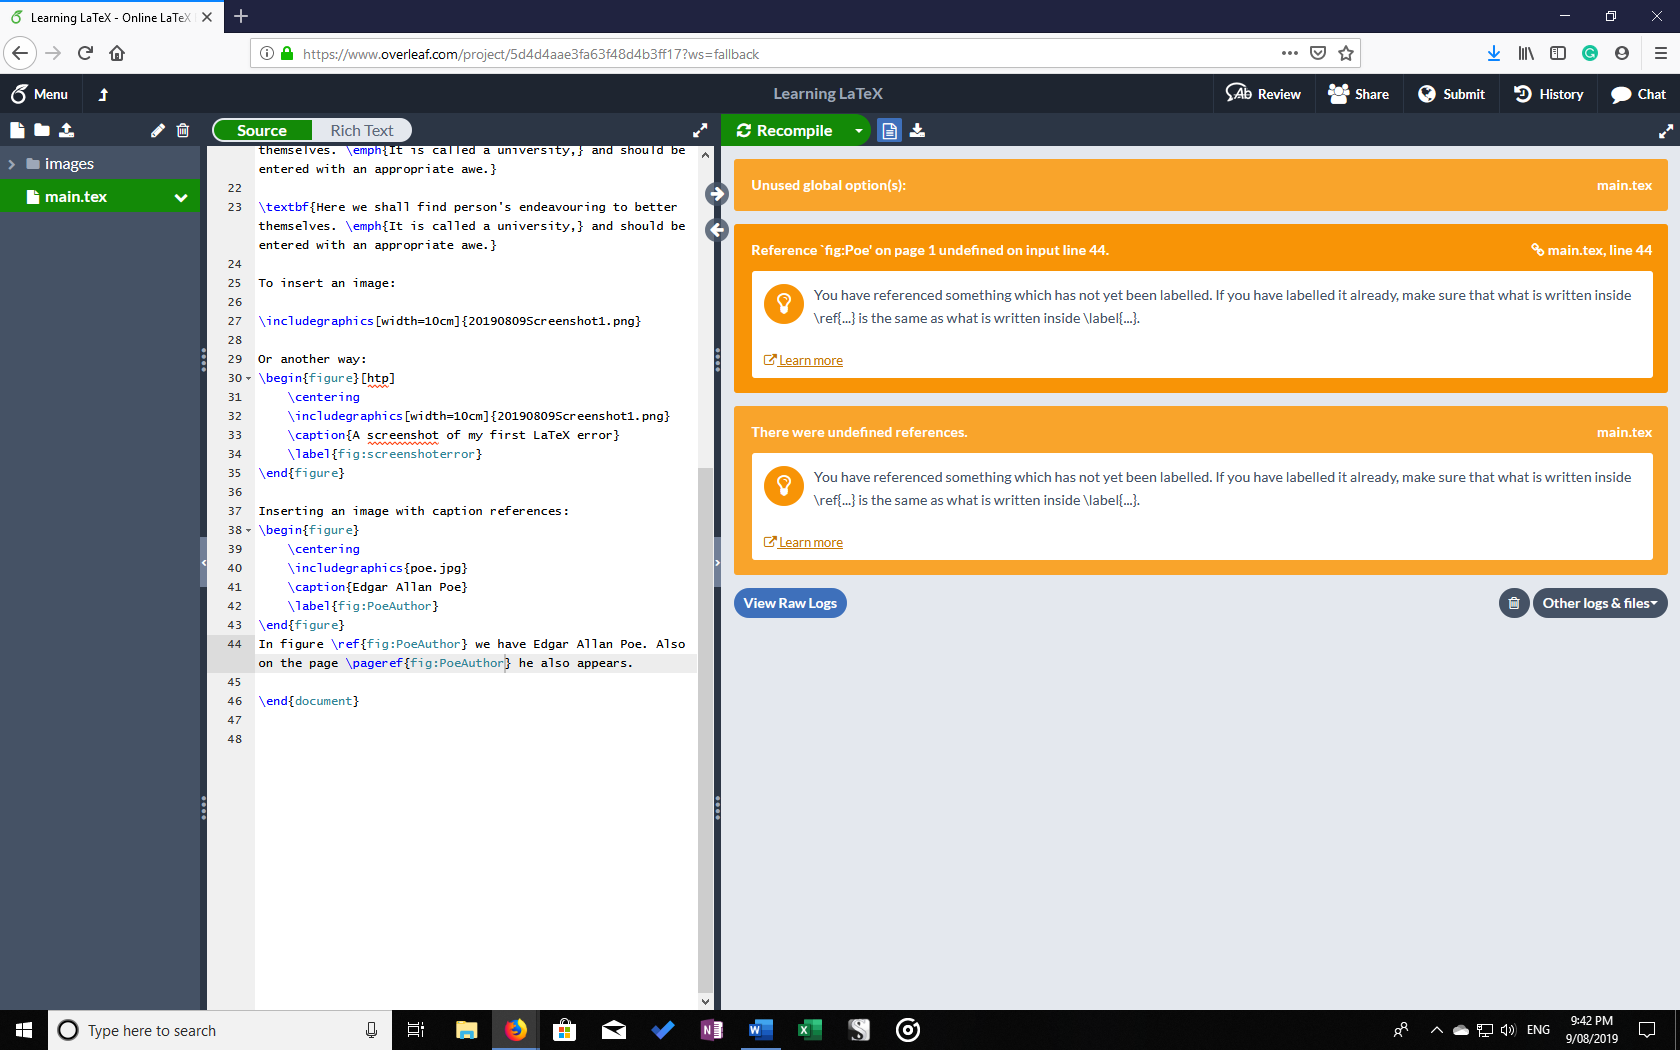
\includegraphics[width=12cm]{Images/Screenshot7.png}
    \caption{Resolving error messages}
    \label{fig:screenshot7}
\end{figure}

\begin{figure}[h]
    \centering
    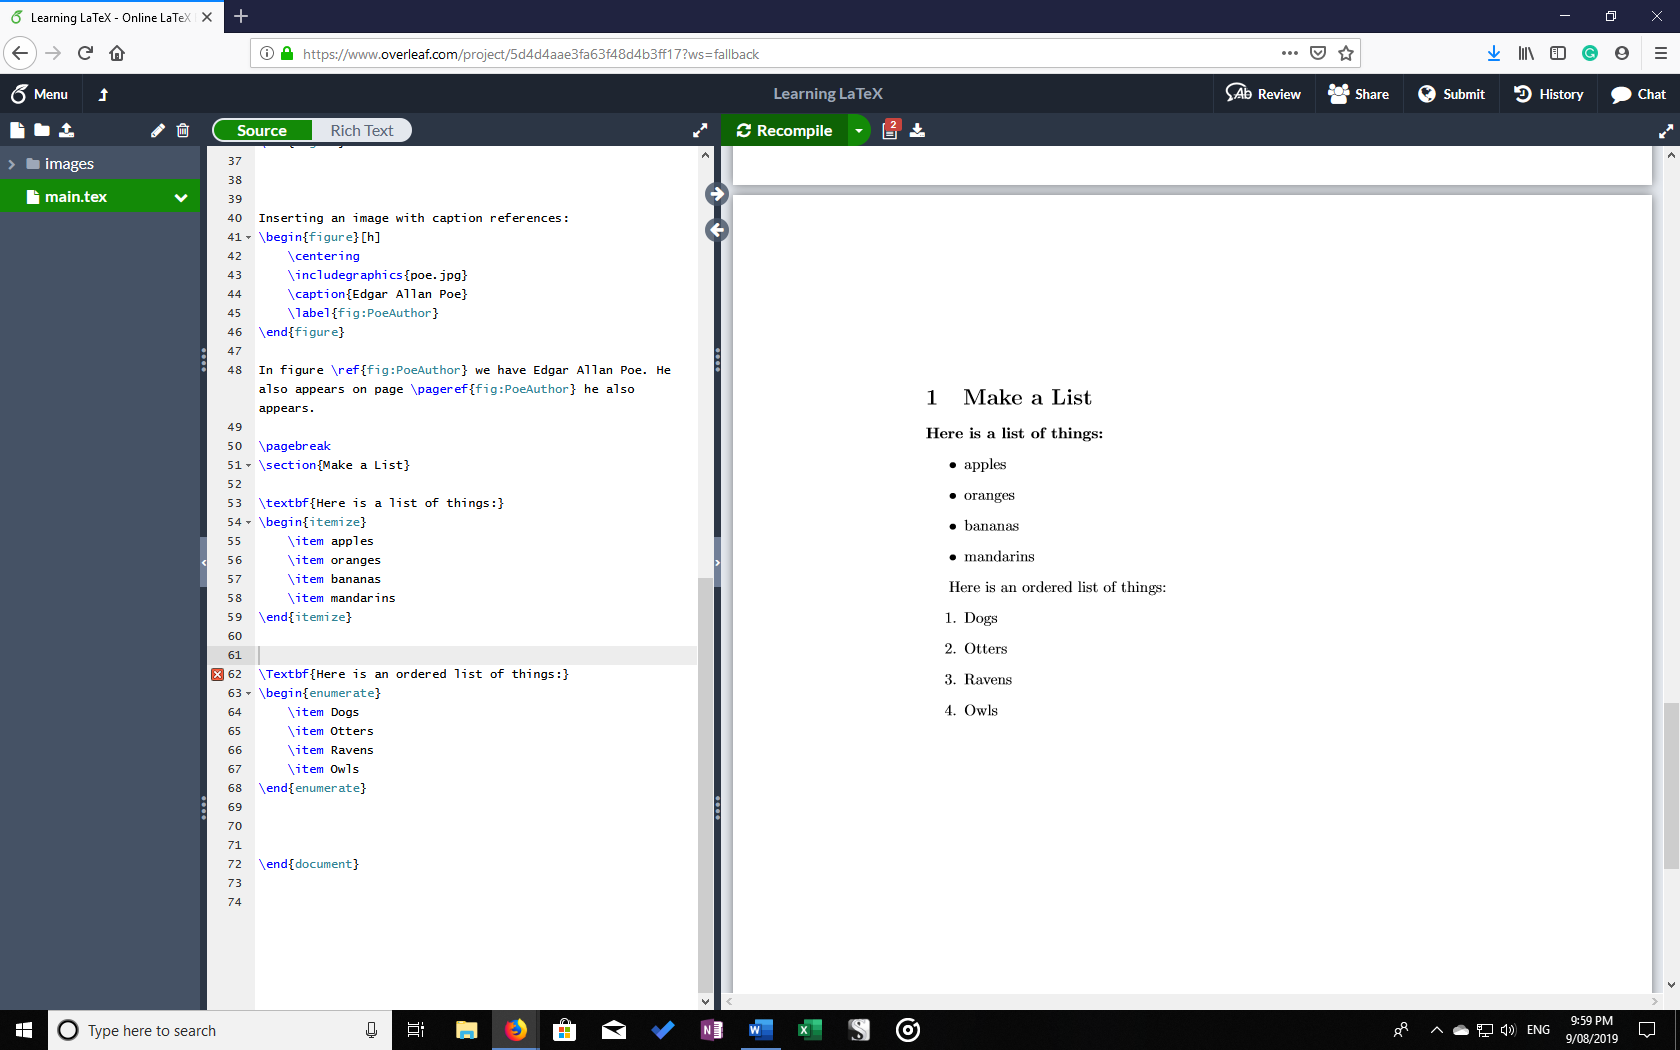
\includegraphics[width=12cm]{Images/Screenshot8.png}
    \caption{Caption}
    \label{fig:Making a list}
\end{figure}

\begin{figure}[h]
    \centering
    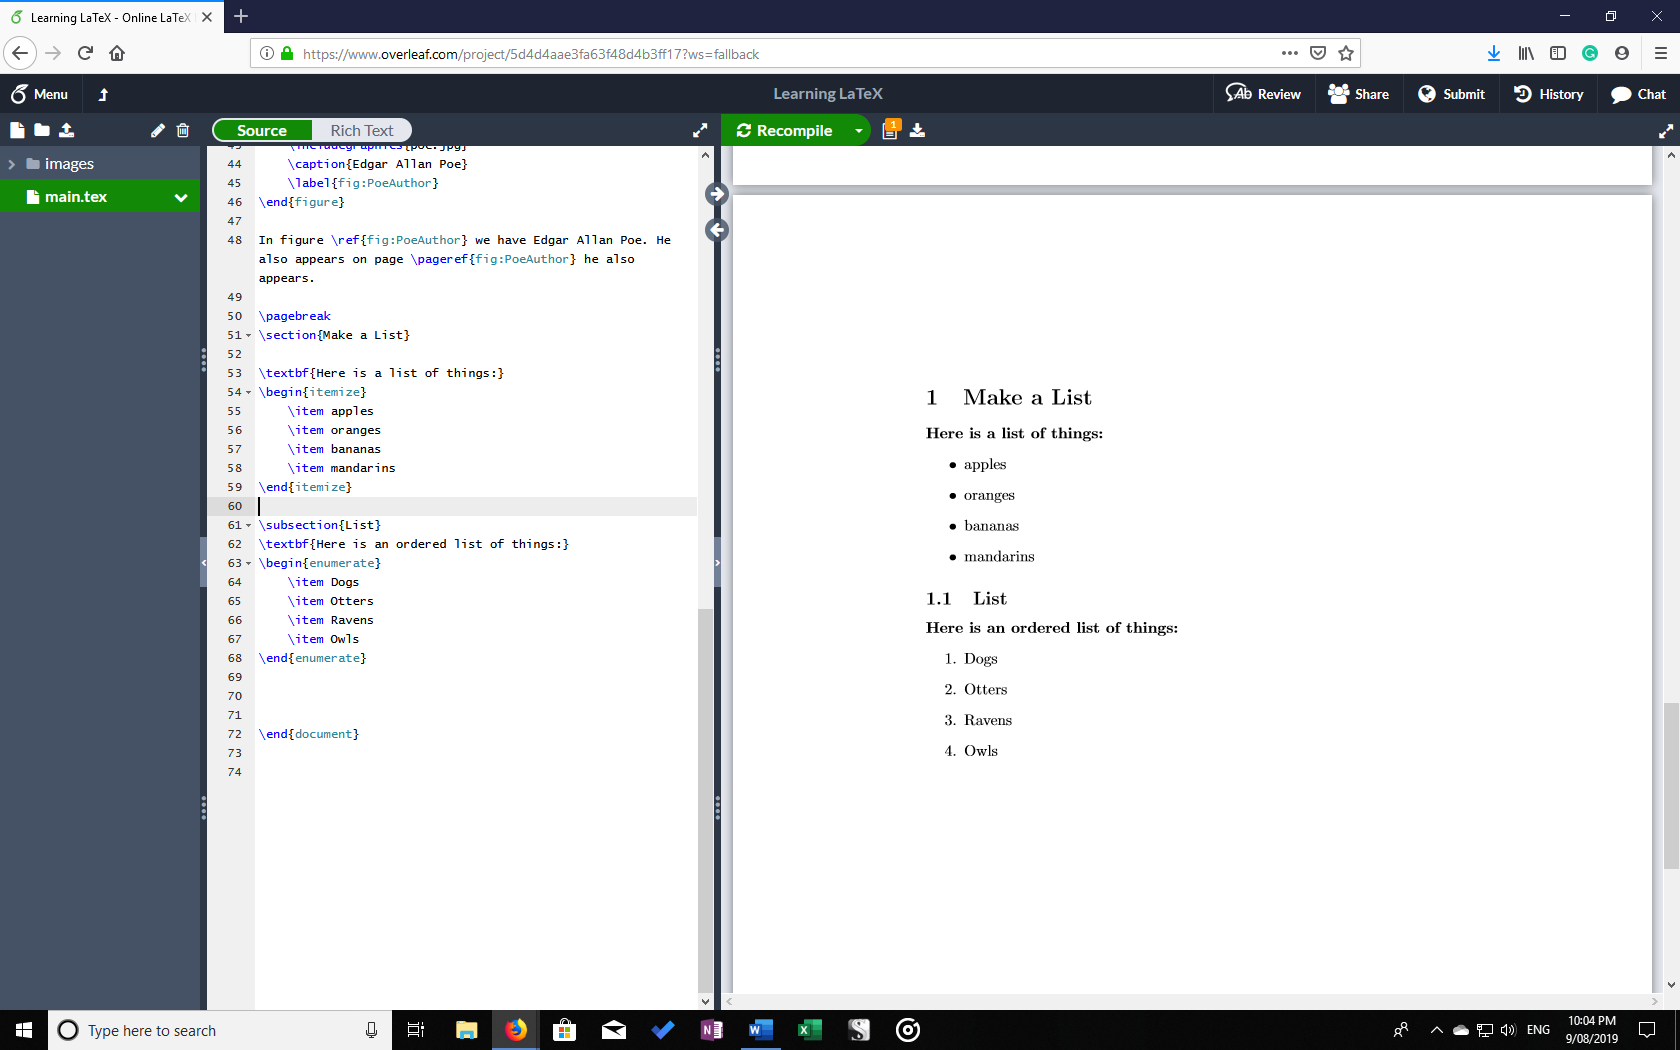
\includegraphics[width=12cm]{Images/Screenshot9.png}
    \caption{Caption}
    \label{fig:Making a subsection}
\end{figure}

\begin{figure}[h]
    \centering
    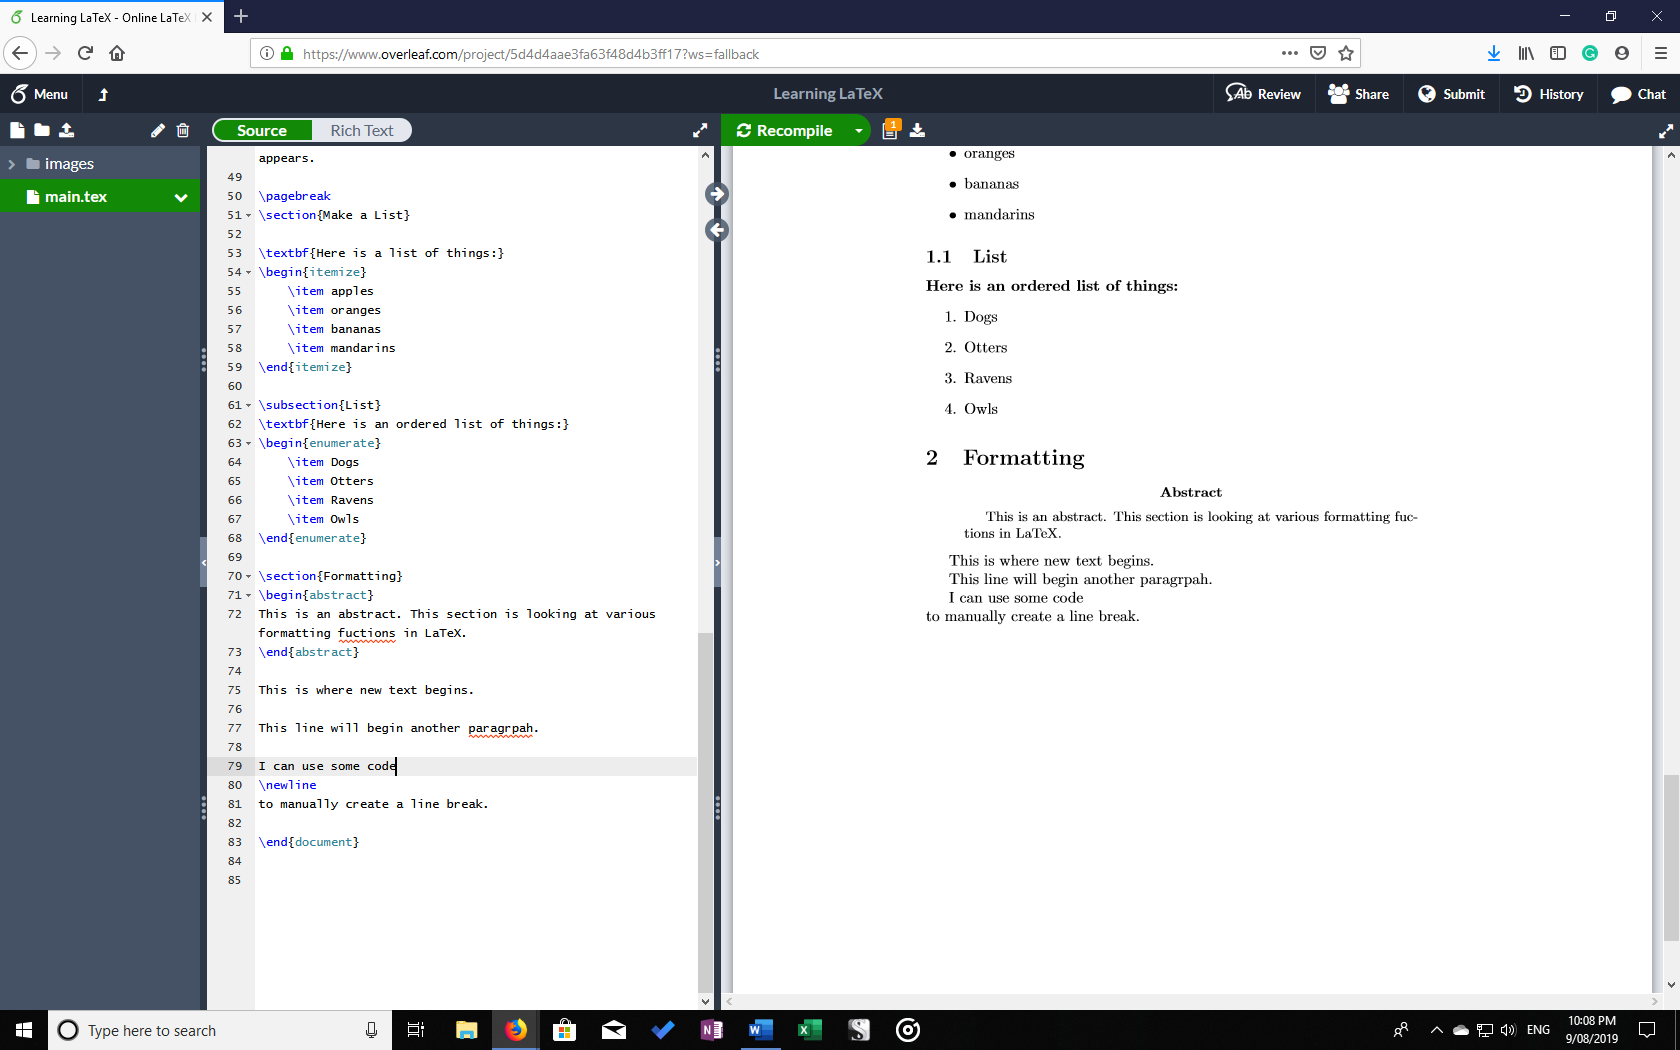
\includegraphics[width=12cm]{Images/Screenshot10.png}
    \caption{Text style formatting}
    \label{fig:screenshot10}
\end{figure}

\begin{figure}[h]
    \centering
    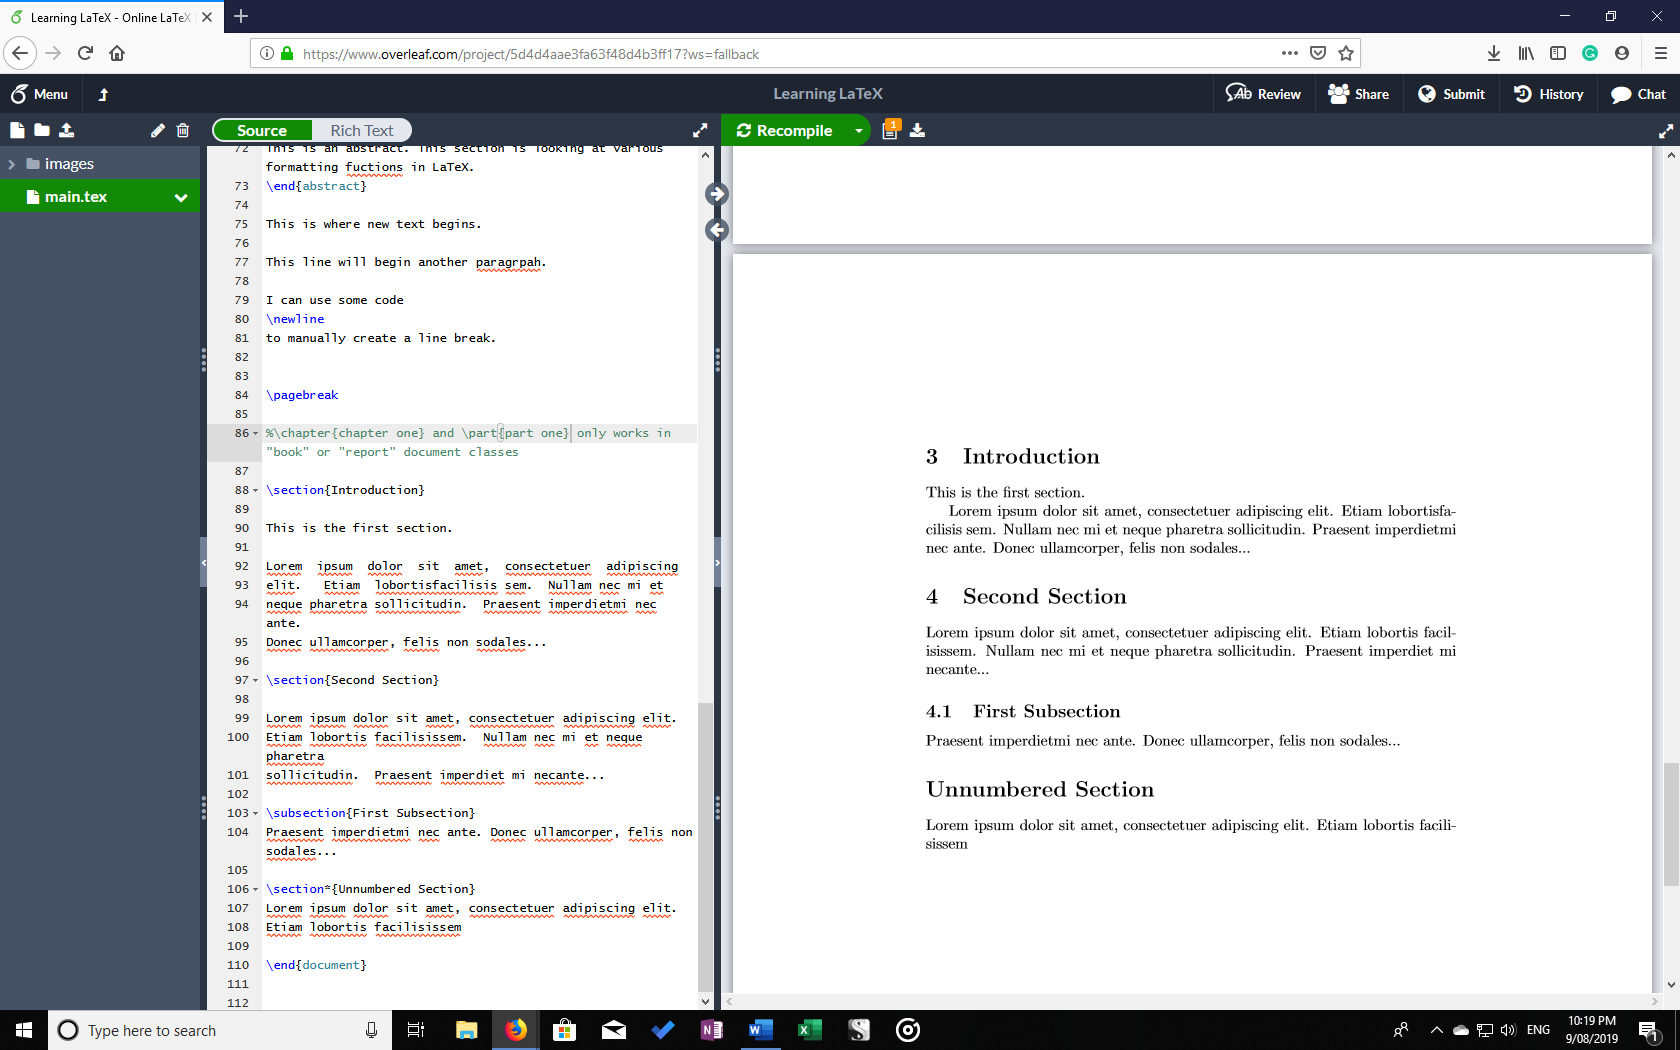
\includegraphics[width=12cm]{Images/Screenshot11.png}
    \caption{Section formatting}
    \label{fig:screenshot11}
\end{figure}

\end{document}
